\chapter{Structures atomiques, de l'hélium aux atomes complexes}
\section{Systèmes héliumnoïdes}
\subsection{Hamiltonien biélectronique}
Un système est héliumoïde lorsqu'il ne possède que deux électrons ($H^-, He, Li^+, Be^{2+},\dots 
U^{90+}$). L'hamiltonien d'un tel système est donné par\\

\retenir{\begin{equation}
H = - \frac{\hbar^2}{2 {\color{blue}\mu}} \sum_{i=1}^2 \nabla_{r_i}^2- \sum_{i=1}^2 \frac{Ze^2}{(4 \pi \epsilon_0) r_i}
{\color{red}
+  \frac{e^2}{(4 \pi \epsilon_0) r_{12} } }
- \frac{\hbar^2}{ {\color{blue} M}} \mbox{\boldmath $ \nabla $}_{r_1}
\cdot \mbox{\boldmath $ \nabla $}_{r_2}
\end{equation}}\ \\

L'avant dernier terme est la répulsion coulombienne entre les deux électrons et le dernier terme dépend
de la masse du noyau, mais également de la position des électrons. Il va se manifester lors de la
comparaison des isotopes (déplacement des raies spectrales. Cet effet ne se manifeste que lorsque l'on
a plus d'un électron). Pour attaquer l'équation de \textsc{Schrödinger} $H \psi ( {\bf r}_1, {\bf r}
_2 ) = E \; \psi ( {\bf r}_1, {\bf r}_2 )$ nous n'en tiendrons pas compte grâce à l'approximation du
\textit{noyau de masse infinie}\footnote{Mais il faut savoir que ça existe.}
\begin{equation}
{\color{blue} M = \infty} \Rightarrow \left\{
\begin{array}{l}
\mu = m \\
(- \frac{\hbar^2}{M}) \mbox{\boldmath $ \nabla $}_{r_1}
\cdot \mbox{\boldmath $ \nabla $}_{r_2} = 0
\end{array}
\right.
\end{equation}

\subsection{Modèle hydrogénoïde et réalité}
Imaginons que l'hamiltonien se limite à la somme des hamiltoniens de chaque particule individuelle
\begin{equation}
H = \overbrace{h(1) + h(2)}^{H^0}
\end{equation}
Sachant que les énergies sont données par $E=-Z^2/2m^2$ et que chaque électron est dans l'état $1s$
qui correspond à $E_1=-4/2*1^2=-2$ u.a. : spectre de $He^+$. En tenant compte du second électron, 
l'énergie est de -4 u.a. (négatif car il s'agit d'une énergie de liaison). Lorsque l'on arrive à
zéro (graphique ci-dessous, à gauche) on forme de l'He$^{++}$.\\

En réalité, nous avons un terme en $r_{12}$ qui vient s'ajouter
\begin{equation}
H = \overbrace{h(1) + h(2)}^{H^0} \hspace*{1cm}
{\color{red}  + \frac{e^2}{4 \pi \epsilon_0 r_{12}}}
\end{equation}
Ce terme provoque une remontée du niveau fondamental d'une trentaine d'eV $${\color{red} \Delta E =
-2.9 - (-4)= +1.1~\mbox{a.u.} \simeq 30~\mbox{eV} }$$ Ceci est l'effet de la paire d'électron via
$r_{12}$. Il n'y a pas contre pas de changement de référence pour $He^+$. Ceci est visible sur le 
graphique ci-dessous, à droite.
\begin{center}
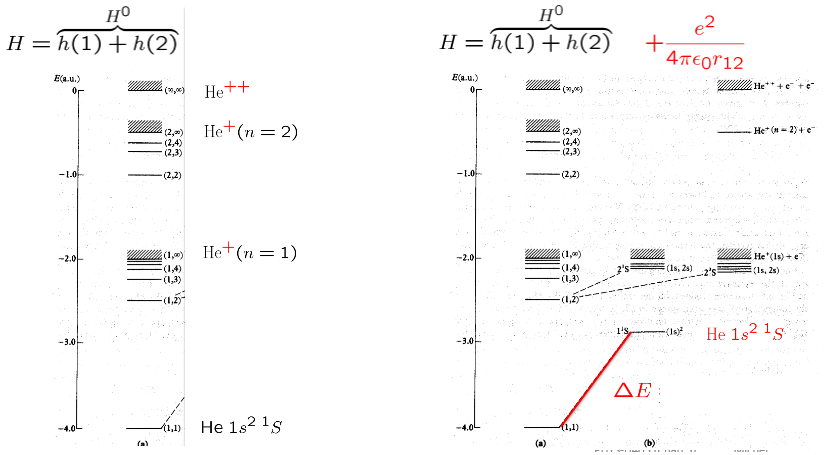
\includegraphics[scale=0.6]{ch3/image1}
\end{center}


\subsection{Écart au potentiel central de Coulomb}
	\begin{wrapfigure}[10]{r}{7cm}
	\vspace{-7mm}
	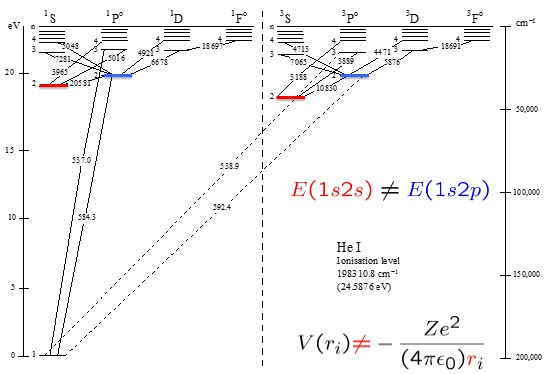
\includegraphics[scale=0.5]{ch3/image2}
	\captionof{figure}{ }
	\end{wrapfigure}

Lors de l'étude de l'hydrogène, nous avions vu que l'énergie ne dépendant que de $n$ et pas de 
$l$ : c'était un "accident" dû au potentiel coulombien (dépendance en $1/r$).\\

 Cependant, dans le 
spectre de l'hélium, l'état $1s2s$ n'a \textbf{pas} la même énergie que $1s2p$ et ce dans l'état
singulet \textbf{et} triplet ! Il semblerait donc que l'énergie dépende de $l$ : l'interaction 
va faire que l'on a plus un potentiel coulombien.\\
\ \\

Lorsqu'un électron se rapproche de noyau ($r=\infty\to r=0$), la charge qu'il ressent change à 
cause de l'effet d'écran : le potentiel n'est plus combombien (passage de $-1/r\to -2/r$)
\begin{equation}
H = h {\color{red} '} (1) 
+ h {\color{red} '} (2) \rightarrow E 
= \epsilon{\color{red} '} _{n_1} 
+ \epsilon{\color{red} '} _{n_2}
\; \; \mbox{avec} \; \; \epsilon{\color{red} '}_n 
= - ({\color{red} Z - \sigma})^2 / 2n^2
\end{equation}

\subsection{Rôle du spin}
Considérons l'hamiltonien du système en u.a.\footnote{A l'examen, c'est quasi toujours faux.}, soit 
celui de deux électrons dans le champ de $Z$ protons\ \\
\retenir{\begin{equation}
H = 
- \frac{1}{2} \nabla_{r_1}^2
- \frac{1}{2} \nabla_{r_2}^2
-  \frac{Z}{r_1} -  \frac{Z}{r_2} 
{\color{red} +  \frac{1}{ r_{12} } }
\end{equation}}\\\

En observant la structure de $H$, on peut voir que l'inversion de $r_1$ et $r_2$ ne change rien 
(ceci n'a rien à voir avec la partité, on a juste changé les indices (indiscernabilité). En 
définissant l'opérateur de permutation $P_{12} \; \psi ( {\bf r}_1, {\bf r}_2 ) \equiv  \psi ( {\bf r}
_2, {\bf r}_1 )$, on a retrouve le commutateur suivant
\begin{equation}
[ H, P_{12} ] = 0 \Rightarrow P_{12} \; \psi ( {\bf r}_1, {\bf r}_2 )
= \lambda \psi ( {\bf r}_1, {\bf r}_2 )
\end{equation}
En appliquant à nouveau cet opérateur
\begin{equation}
P_{12}^2 \; \psi ( {\bf r}_1, {\bf r}_2 ) = \lambda^2
\; \psi ( {\bf r}_1, {\bf r}_2 ) = \; \psi ( {\bf r}_1, {\bf r}_2 ) \quad \Rightarrow\quad
\lambda = \pm 1\quad\Rightarrow\quad \psi_{\pm} ( {\bf r}_1, {\bf r}_2 )
\end{equation}
Ceci nous montre que la fonction sera soit symétrique, soit antisymétrique
\begin{equation}
\left\{ 
\begin{array}{lll}
\lambda = +1 & \mbox{fct spatiale sym\'etrique} & \mbox{(para)} \\
\lambda = -1 & \mbox{fct spatiale anti-sym\'etrique} & \mbox{(ortho)} 
\end{array}
\right.
\end{equation}\ \\

Ayant à disposition les deux commutateurs $[H, {\bf S}^2 ] = [H, S_z ] = 0$, il est possible de 
définir une base \textsc{ecoc} \ \\

\retenir{\begin{equation}
\mbox{Base ECOC}~\{ {\bf S}_1^2, {\bf S}_2^2,   {\bf S}^2,  S_{z} \}
\Rightarrow \{ \vert S_1 S_2 S M_S \rangle \}
\end{equation}}\ \\

En effet, en utilisant la relation de fermeture on peut écrire
\begin{equation}
\begin{array}{ll}
\DS\ket{\frac{1}{2}\frac{1}{2}SM_S} &\DS= \sum_\alpha \ket{\alpha}\bra{\alpha}\ket{\frac{1}{2}\frac{1}
{2}SM_S}\\
&\DS= \sum_{m_{S1}m_{S2}} \ket{S_1^2 = \frac{1}{2}, S_{z1} = m_{S1}, S_2^2 = \frac{1}{2}, S_{z2} = m_{S2}}\bra{\frac{1}{2}m_{S1}\frac{1}{2}m_{S2}}\ket{\frac{1}{2}\frac{1}{2}SM_2}
\end{array}
\end{equation}
où $M_S=m_{S1}+m_{S2}$.\\

En couplant deux spin $1/2$, on peut avoir $S=0,1$ : état singulet (bleu, $M_S=0$) ou triplet (rouge,
$M_S=0,\pm1$)
\begin{equation}
\left\{
\begin{array}{ll}
\vert \frac{1}{2}\frac{1}{2}   {\color{red} 1 }+1 \rangle  & = \alpha(1) \alpha(2) \\
\vert \frac{1}{2}\frac{1}{2}   {\color{red} 1 } 0 \rangle   & = \frac{1}{\sqrt{2}} [ \alpha(1) \beta(2) + \beta(1) \alpha(2) ] \\
\vert \frac{1}{2}\frac{1}{2}   {\color{red} 1 } -1 \rangle   & = \beta(1) \beta(2) \\
\vert \frac{1}{2}\frac{1}{2}   {\color{blue} 0 } 0 \rangle   & =\frac{1}{\sqrt{2}} [ \alpha(1) \beta(2) - \beta(1) \alpha(2) ] \\
\end{array} \right.
\end{equation}
Le premier triplet $(M_S=1)$ doit forcément être composé de deux spin \textit{up} (car $M_S=\sum
m_s$) tandis que le troisième $(M_S=-1)$ doit être deux spin \textit{down} pour les mêmes raisons.\\

Comment interpréter le second et le dernier triplet ? Il s'agit d'un mélange de \textit{up} et 
\textit{down}. Nous avons cette combinaison linéaire tout simplement à l'aide des coefficients
de Clebsh-Gordan dû au changement d'\textsc{ecoc}. Mieux encore : on peut le retrouver à l'aide
des opérateurs élévateurs et abaisseurs couplés $S_\pm$. Considérons le premier triplet
\begin{equation}
\ket{\frac{1}{2}\frac{1}{2}0(+1)} = \alpha(1)\alpha(2)
\end{equation}
Appliquons-lui l'opérateur élévateur et abaisseur "totaux"
\begin{equation}
[S_-(1)+S_-(2)]\alpha(1)\alpha(2) = \beta(2)\alpha(2)+\alpha(1)\beta(2)
\end{equation}
On retrouve alors le second triplet
\begin{equation}
\ket{\frac{1}{2}\frac{1}{2}01} = 0*\alpha(2)\alpha(2) + \frac{1}{\sqrt{2}}\beta(1)\alpha(2) + 
\frac{1}{\sqrt{2}}\alpha(1)\beta(2) + 0*\beta(1)\beta(2)
\end{equation}
Il est possible de retrouver le quatrième triplet par orthogonalité dans le sous-espace $M_S$.\\

Intéressons-nous maintenant à la représentation matricielle de $S_z$ et $\vec{S}^2$
\begin{equation}
S_z = \hbar  \left( \begin{array}{cccc}
{\color{red} +1 } &  0  &  0  &  0  \\
0    &  {\color{red} 0 }   &  0  &  0  \\
0    &  0  &  {\color{red} -1 }   &  0  \\
0    &  0  &  0  & {\color{blue} 0 }  \end{array} \right),\qquad\qquad
{\bf S}^2 = \hbar^2  \left( \begin{array}{cccc}
{\color{red} 2 } &  0  &  0  &  0  \\
0    &  {\color{red} 2 }  & 0 &  0  \\
0    &  0  & {\color{red} 2 } &  0  \\
0    &  0  &  0  & {\color{blue} 0 } \end{array} \right)
\end{equation}
Les valeurs propres de $\vec S^2$ (valant $s(s+1)$) sont trois fois 2 et une fois 0. Il n'est pas
possible de les dinstinguer seulement avec cette représentation. Heureusement $S_z$, via la valeur
de $m_s$ va permettre de les identifier. Nous avons ainsi deux opérateurs qui spécifient totalement
l'état de spin : la représentation dans la base couplée est orthogonale (ce qui n'est pas le cas dans
la base découplée). Le changement d'\textsc{ecoc} diagonalise les opérateurs.


\subsection{Postulat de symétrisation}

	\begin{wrapfigure}[13]{r}{7cm}
	\vspace{-7mm}
	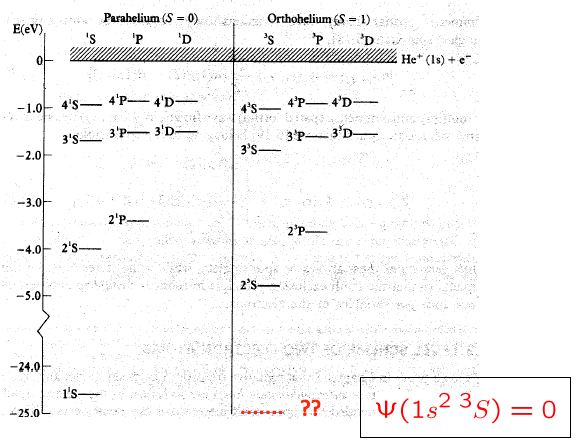
\includegraphics[scale=0.5]{ch3/image3}
	\captionof{figure}{ }
	\end{wrapfigure}

Nous avons constaté expérimentalement que l'état $1s^2$ n'existe pas dans l'orthohélium ($S=1$, 
triplet). Il a fallu postuler quelque chose afin que cet état s'annule pour que les résultats
théoriques collent aux résultats expérimentaux. C'est ainsi que le postulat d'antisymétrisation a
été proposé : la fonction d'onde des électrons (fermions) devra être antisymétrique à l'échange. Ceci
est vérifié dans le cas singulet
\begin{equation}
\underbrace{1s(\bf{r}_1)1s(\bf{r}_2)}_{\text{spatial sym.}}
\frac{1}{\sqrt{2}} 
\underbrace{ \alpha(1) \beta(2) - \beta(1) \alpha(2) ]}_{\text{singulet antisym.}}
\end{equation}
Écrivons la même relation pour le cas où $S=1$
\begin{equation}
{\color{red}
\underbrace{1s(\bf{r}_1)1s(\bf{r}_2)}_{\text{spatial sym.}}
\frac{1}{\sqrt{2}} 
\underbrace{ \alpha(1) \beta(2) + \beta(1) \alpha(2) ] = 0 }_{\text{triplet sym.}}}
\end{equation}
Le postulat d'antisymétrie implique que cette fonction d'onde soit nulle car, étant symétrique, elle
ne respecte pas le postulat. On peut essayer de rendre la partie spatiale anti-symétrique mais le
constat est que celle-ci s'annulera :
\begin{equation}
1s(r_1)1s(r_2) - s1(r_2)1s(r_1) = 0
\end{equation}\ 

Ainsi, \textbf{la fonction d'onde totale d'un système de $N$ électrons (fermions!) doit être 
antisymétrique par rapport à l'échange}\ \\

\cadre{\begin{equation}
P_{12} \; \Psi (q_1,q_2) \equiv  \Psi ( q_2, q_1) = - \Psi (q_1, q_2)
\end{equation}}\ \\

Ceci va imposer un couplage entre les variables d'espace et de spin. Pour les états triplets 
($S=1$) ou \textit{ortho}
\begin{equation}
\Psi (q_1,q_2) = \psi_{\color{red} - } ( {\bf r}_1, {\bf r}_2 ) \times
\left\{
\begin{array}{l}
\alpha(1) \alpha(2) \\
\frac{1}{\sqrt{2}} 
[ \alpha(1) \beta(2) + \beta(1) \alpha(2) ] \\
\beta(1) \beta(2) 
\end{array} \right.
\end{equation}
Pour les états singulets ($S=0$) ou \textit{para}
\begin{equation}
\Psi (q_1,q_2) = \psi_
{\color{blue} +}  ( {\bf r}_1, {\bf r}_2 ) \times
\frac{1}{\sqrt{2}} 
[ \alpha(1) \beta(2) - \beta(1) \alpha(2) ]
\end{equation}

Ceci peut s'écrire à l'aide des spin-orbitales
\begin{equation}
\Psi_{LM_LSM_S}(q_1,q_2) = \psi_{LM_L}( {\bf r}_1, {\bf r}_2) 
\chi_{SM_S}(1,2)
\end{equation}
On en tire les contraintes de la symétrie d'échange\footnote{Rappelons que dans un système à deux
électrons, on peut faire une rotation autour de n'importe quel noyau seulement pour $J$.}\\

\cadre{\begin{itemize}
\item[$\bullet$] Triplet ($S=1, M_S =+1,0,-1$)
\begin{equation}
\Psi_{LM_LSM_S}(q_1,q_2) = 
\psi^{\color{red} -}_{LM_L}( {\bf r}_1, {\bf r}_2) 
\chi^{\color{blue} +}_{1M_S}(1,2)
\end{equation}
\item[$\bullet$] Singulet ($S=0,M_S=0$)
\begin{equation}
\Psi_{LM_LSM_S}(q_1,q_2) = 
\psi^{\color{blue} +}_{LM_L}( {\bf r}_1, {\bf r}_2) 
\chi^{\color{red} -}_{00}(1,2)
\end{equation}
\end{itemize}}\ \\

Fort de nos nouvelles connaissances, écrivons proprement un \textit{ket} de façon complète
\begin{equation}
\vert \{ nl n'l' \} L M_L S M_S \rangle = 
\frac{1}{\sqrt{2}} [
  \vert nl(1) n'l'(2) L M_L S M_S \rangle
{\color{red} - }
\vert nl(2) n'l'(1) L M_L S M_S \rangle ]
\end{equation}
où le crochet signifie \textit{configuration électronique} (insiste sur le fait que l'on ne sait pas
ou se trouve (1) et (2)), où le "-" garanti l'antisymétrie et ou (par exemple) $ nl(1) n'l'(2)$ 
est un état couplé dans lequel se cache un Clebsh-Gordan. Deux électrons de spin $1/2$ se regroupent
ainsi dans $S$ de projection $M_S$ : il faut envisager les deux possibilités mais \textbf{attention}
l'ordre de couplage (spin-orbite ou orbite-spin) est \textbf{important}\footnote{On en parle plus 
tard} !\\

Il faut donc envisager deux possibilités
\begin{enumerate}
\item $S = 1 ~\mbox{triplet} ~\Rightarrow 
\psi^-_{LM_L}( {\bf r}_1, {\bf r}_2) 
\chi^+_{1M_S}(1,2)$
\item $S=0 ~\mbox{singlet}~ \Rightarrow
\psi^+_{LM_L}( {\bf r}_1, {\bf r}_2) 
\chi^-_{00}(1,2)$
\end{enumerate}\ 

Regardons les termes $LS$ découlant d'une configuration $1snl$
\begin{equation}
\begin{array}{ll}
1s nl  &\rightarrow  {\bf L} = {\bf 0}+ {\bf l}  \rightarrow L=l\\
&\rightarrow {\bf S} = {\bf 1/2}+ {\bf 1/2} 
 \rightarrow S=1,0
\end{array}\qquad \qquad \left\{
\begin{array}{l}
^1L \\
^3L
\end{array}
\right.
\end{equation}

\exemple{ Voir notes.
\begin{equation}
\begin{array}{lll}
1s 2s & \rightarrow  &  ^1S, \; ^3S  \\
1s 2p & \rightarrow  &  ^1P^o, \; ^3P^o  \\
1s 3d & \rightarrow  &  ^1D, \; ^3D  \\
1s 4f & \rightarrow  &  ^1F^o, \; ^3F^o  \\
\end{array}
\end{equation}}

\subsection{Termes et déterminants de Slater}
Dans un déterminant de \textsc{Slater}, on n'écrit pas explicitement la partie sptiale et celle de 
spin car on construit une spin-orbitale. La partie spatiale et de spin sont alors intriquées
\begin{equation}
\vert a b \vert \equiv \frac{1}{\sqrt{2!}} \;
\left\vert
\begin{array}{cc}
a(q_1) & b(q_1) \\
a(q_2) & b(q_2)
\end{array}
\right\vert
= \frac{1}{\sqrt{2!}} [ a(q_1) b(q_2) -  a(q_2) b(q_1) ]
\end{equation}
Voyons comment écrire un état singlet
\begin{equation}
\mbox{Singlet} \Rightarrow 
\Psi_{LM_LSM_S}(q_1,q_2) = 
\psi^{\color{blue} +}_{LM_L}( {\bf r}_1, {\bf r}_2) 
\chi^{\color{red} -}_{00}(1,2)
\end{equation}
On recherche donc à exprimer $\psi^{+}_{00}( {\bf r}_1, {\bf r}_2)  \chi^{-}_{00}(1,2)$ sous la forme
d'un déterminant de \textsc{Slater}
\begin{equation}
\begin{array}{ll}
\Psi (1s^2 \; ^1S_{0,0}) 
&\DS= \underbrace{1s( {\bf r}_1) 1s ({\bf r}_2)}_{\text{spatial}} \frac{1}{\sqrt{2}}\underbrace{  [\alpha(1) \beta(2) - \beta(1) \alpha(2) ]}_{\text{spin}}
\vspace{2mm}\\
&\DS = \frac{1}{\sqrt{2}} \underbrace{[ 1s(1) \overline{1s}(2) - 1s(2) \overline{1s}(1) ]}
_{\text{spin-orbite}}
=  \vert 1s \overline{1s} \vert
\end{array}
\end{equation}
où le passage à la deuxième ligne s'effectue via $\alpha\to 1s, \beta\to \bar{1s}$.\\

Nous avons exprimé l'état avec \textbf{un} déterminant de \textsc{Slater}, mais ce n'est pas toujours
le cas. Refaisons le même exercice avec $1s2p$ ($^1P^o_{0,0}$ veut dire \textit{singlet P, S=0, 
puis $M_L,M_S$} (impair car $(-1)^{\sum\dots}$) : on caractérise bien l'état avec toute ses valeurs
propres). On veut donc écrire $\psi^{+}_{10}( {\bf r}_1, {\bf r}_2)  \chi^{-}_{00}(1,2)$ :
\begin{equation}
\begin{array}{ll}
\Psi(1s2p \; ^1P^o_{0,0})&\DS = 
 \frac{1}{\sqrt{2}} [1s( {\bf r}_1) 2p_0 ({\bf r}_2) +
1s( {\bf r}_2) 2p_0 ({\bf r}_1) ]\times
 \frac{1}{\sqrt{2}}  [\alpha(1) \beta(2) 
- \beta(1) \alpha(2) ]\vspace{2mm}\\
&\DS = \frac{1}{\sqrt{2}}  
\left[
\vert 1s \overline{2p}_0 \vert
-
\vert \overline{1s} 2p_0 \vert
\right]
\end{array}
\end{equation}
Il s'agit donc d'une \textbf{combinaison} de déterminants de \textsc{Slater}, deux pour être précis 
!\\

On peut continuer l'exercice avec l'état triplet
\begin{equation}
\mbox{Triplet} \Rightarrow 
\Psi_{LM_LSM_S}(q_1,q_2) = 
\psi^{\color{red} -}_{LM_L}( {\bf r}_1, {\bf r}_2) 
\chi^{\color{blue} +}_{1M_S}(1,2)
\end{equation}
Cette fois, on veut exprimer $\psi^{-}_{10}( {\bf r}_1, {\bf r}_2)  \chi^{+}_{1-1}(1,2)$. Même 
exercice
\begin{equation}
\begin{array}{ll}
\Psi(1s2p \; ^3P^o_{0,-1}) &\DS= 
 \frac{1}{\sqrt{2}} [1s( {\bf r}_1) 2p_0 ({\bf r}_2) - 
1s( {\bf r}_2) 2p_0 ({\bf r}_1) ] \beta(1) \beta(2)\\
&\DS = \frac{1}{\sqrt{2}} 
[ \overline{1s}(1) \overline{2p}_0(2) 
- \overline{1s}(2) \overline{2p}_0(1) ]
=\vert \overline{1s} \overline{2p}_0 \vert
\end{array}
\end{equation}
Pour avoir $M_M=0$ et $M_S=-1$, c'est le seul état possible : ils doivent tous être antisymétriques.

\subsection{Principe de Pauli en action}
Aussi bizarre que cela puisse paraître, l'ordre de couplage (spin-orbite ou orbite-spin) a de 
l'importance (au niveau de la phase). En bref $j_1+j_2 \neq j_2+j_1$ ! On pourrait croire que ce n'est
pas grave mais ça l'est pour l'indiscernable des électrons
\begin{equation}
\vert \overbrace{j_1 j_2}^{\alpha} j m \rangle = 
{\color{red} 
(-1)^{j_1 + j_2 -j}    }
\vert \overbrace{j_2 j_1}^{\beta}j m \rangle
\end{equation}
En résumé, \textbf{attention à l'ordre du couplage des moments angulaires!}\\

Construisons une fonction \textbf{antisymétrique} pour l'échange
\begin{equation}
\begin{array}{ll}
\vert \{ nl n'l' \} L M_L S M_S \rangle &\DS= 
\frac{1}{\sqrt{2}} [
  \vert nl(1) n'l'(2) L M_L S M_S \rangle
{\color{red} - }
\vert nl(2) n'l'(1) L M_L S M_S \rangle ]\\
&\DS= 
\frac{1}{\sqrt{2}} [R_{nl}(r_1) R_{n'l'}(r_2)
  \vert l(1) l'(2) L M_L S M_S \rangle
-
R_{nl}(r_2) R_{n'l'}(r_1)
\vert {\color{blue} l(2) l'(1) } L M_L S M_S \rangle ]\\
&\DS= 
\frac{1}{\sqrt{2}} [R_{nl}(r_1) R_{n'l'}(r_2)
  \vert l(1) l'(2) L M_L S M_S \rangle\\
  &\qquad\qquad- 
\underbrace{\color{red} (-1)^{l+l'-L}(-1)^{1/2+1/2-S} }_{\danger\ \text{ordre couplage}}
R_{nl}(r_2) R_{n'l'}(r_1)
\vert {\color{blue} l'(1) l(2) }  L M_L S M_S \rangle ]
\end{array}
\end{equation}
Le principe de \textsc{Pauli} rentre en actions pour les électrons \textbf{équivalents} ($nl=n'l'$).
Si c'est le cas, on peut mettre $R_{nl}(r_1)$ et $R_{nl}(r_2)$ en évidence. Se faisant, il apparaît un
facteur numérique qui peut s'annuler dans certaines situations
\begin{equation}
\begin{array}{ll}
\vert \{ nl^2 \} L M_L S M_S \rangle &\DS= 
R_{nl}(r_1) R_{nl}(r_2) \vert  l(1)l(2) L M_L S M_S 
\rangle
\left [ 1 
- (-1)^{2l-L}(-1)^{1-S} \right]\vspace{2mm}\\
&\DS =
R_{nl}(r_1) R_{nl}(r_2) \vert  l(1)l(2) L M_L S M_S 
\rangle
{\color{red} 
\left [ 1 + (-1)^{-L-S} \right] }
\end{array}
\end{equation}
On en tire\\

\cadre{\begin{equation}
\Psi_{nl^2 LM_LSM_S}(q_1,q_2) 
\left\{ \begin{array}{ll}
= 0 & \mbox{si}~(L+S)~ \mbox{impair} \\
\neq 0 & \mbox{si}~(L+S)~ \mbox{pair} \end{array} \right.
\end{equation}}\ \\

	\begin{wrapfigure}[7]{r}{2cm}
	\vspace{-7mm}
	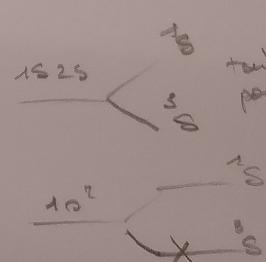
\includegraphics[scale=0.3]{ch3/image4}
	\captionof{figure}{ }
	\end{wrapfigure}
	
Ceci permet de réaliser ce qu'il se passe lorsque deux électrons sont sur la même couche. Ceci 
explique notamment pourquoi il manque l'état fondamental dans l'état triplet : on essaye de créer 
quelque chose d'antistymétrique provoquant une annulation. Cette règle est \textbf{importante} car,
dans certains cas ($Si (L+S)$ est impair pour des électrons équivalents), les "inégalités
triangulaires" ne pourront \textbf{pas} être appliquées! Toutes les configurations proposées par
celles-ci pourront être interdites.\\

Considérons le cas d’électrons non-équivalents ($nl\neq n’l’$) : $1sns$. Un électron peut être placé dans deux boîtes ($1s$ : un électron dans 2 boîtes et $ns$ : un électron dans 2 autres boîtes)
\begin{equation}
1sns \Rightarrow \; ^3S, \; ^1S 
\end{equation}
Comme nous avons deux électrons cela fait 4 (soit dévaluation de la dégénérescence) : on peut avoir du triplet et du singlet
\begin{equation}
g =  \left( \frac{2!}{1!(2-1)!} \right) ^2 = 2^2 = 4 (=3+1)
\end{equation}
Ici, on peut utiliser (et il ne faut pas hésiter) les relations triangulaires mais aussi les 
"sudoku".\\

Si par contre les électrons sont équivalents ($nl = n’l’$)($1s^2$), l'état $^3S$ est interdit. 
\begin{equation}
1s^2 \Rightarrow \; ^3S, \; ^1S
\end{equation}
Il faut en effet que $(L+S)$ soit pair. En évaluant la dégénérescence, il n'y a que l'état singulet qui est possible. 
\begin{equation}
g =   \frac{2!}{2!(2-2)!}  = 1
\end{equation}
On ne peut donc \textbf{pas} appliquer ici les relations triangulaires (algèbre vectoriel).

\begin{center}
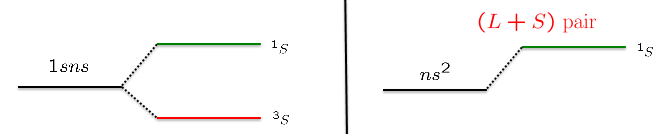
\includegraphics[scale=0.5]{ch3/image5}
\captionof{figure}{A gauche $1sns$ et à droite $1s^2$}
\end{center}
 
On peut compliquer et considérer la différence entre $2p3p$ (électrons non-équivalents) et $2p^2$ électrons équivalents). Dans le premier cas, six boîtes sont disponibles (dégénérescence de spin)
\begin{equation}
2p3p\Rightarrow \; ^3D, \; ^1D, \; ^3P, \; ^1P, \; ^3S, \; ^1S
\end{equation}
Comme nous avons 2 électrons, nous avons 36 cases disponibles. 
\begin{equation}
g =  \left( \frac{6!}{5!(6-1)!} \right) ^2 = 6^2 = 36
\end{equation}
Ce résultat est cohérent : comme nous avons 5 cases spatiales pour $D$, une pour $S$ et trois 
pour $P$, on trouve $15 + 5 + 9 + 3 + 3 + 1=36$.\\

Dans le cas des électrons équivalents, la vie est moins belle : seules les configurations ou ($L+S$) est pair sont autorisées. Il n'y a donc que 15 emplacements possibles : contrait d'utiliser la règle du sudoku.


\begin{center}
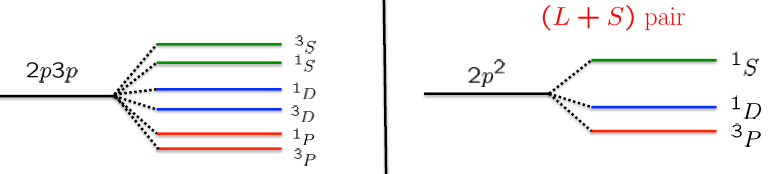
\includegraphics[scale=0.5]{ch3/image6}
\captionof{figure}{A gauche $2p3p$ et à droite $2p^2$}
\end{center} 


\subsection{Répulsion de Coulomb et naissance de termes}
Considérons l'hamiltonien de notre système, exprimé en unités atomiques
\begin{equation}
H = h(1) + h(2) + \frac{1}{r_{12}}
\end{equation}
Celui-ci est clairement indépendant du spin. On peut alors se demande si l'énergie, elle, dépend du spin La réponse est oui, assez étonnamment.\\

Pour comprendre comment cette dépendance en énergie est possible, il est nécessaire d"écrire l"interaction de Coulomb sous forme tensorielle. Ceci est possible grâce au développement en polynômes de Legendre et avec l'aide des harmoniques sphériques
\begin{equation}
\frac{1}{r_{12}} = \sum_k^\infty \frac{r_<^k}{r_>^{k+1}}
P_k (\cos \omega)
\end{equation}
où la signification de $r_{<,>}$ sont des fonctions radiales telles que $r_> > r_<$. Considérons le
théorème d'addition des harmoniques sphériques 
\begin{equation}
P_k (\cos \omega) = 
\frac{4 \pi}{2k+1} \sum_{q=-k}^{+k} \underbrace{Y^\ast_{kq}(\theta_1, \phi_1)}_{\text{HS elec 1}}
\underbrace{Y_{kq}(\theta_2, \phi_2)}_{\text{HS elec 2}}
\end{equation}
où $\omega$ est l'angle entre $r_1$ et $r_2$. Cette somme contient bien $2k+1$ composantes ce qui est cohérent car l'harmonique sphérique est un tenseur de rang $k$ à $2k+1$ composante. Compte-tenu de ce théorème, on peut ré-écrire le terme $1/r_{12}$ (qui est, pour rappel, l'hamiltonien propre à 
l'interaction de Coulomb)
\begin{equation}
\frac{1}{r_{12}} = \sum_k^\infty \frac{r_<^k}{r_>^{k+1}}
\frac{4 \pi}{[k]} \underbrace{\sum_{q=-k}^{+k} Y^\ast_{kq}(\theta_1, \phi_1)
Y_{kq}(\theta_2, \phi_2)}_{\text{P.scal de 2 OTI}}
\end{equation}
Considérons les harmoniques sphériques renormalisées
\begin{equation}
C^{(k)}_q (\theta, \phi)
=  \sqrt{ \frac{4 \pi}{2k+1} } \;
Y_{kq}(\theta_, \phi_)
\end{equation}
On peut ré-écrire la précédente expression
\begin{equation}
\frac{1}{r_{12}} 
= \sum_k^\infty \frac{r_<^k}{r_>^{k+1}}
 \sum_{q=-k}^{+k} (-1)^q \; C^{(k)}_{-q} (\theta_1, \phi_1)
C^{(k)}_q (\theta_2, \phi_2)
\end{equation}
où $(-1)^q$ est la signature de $Y^*$. En utilisant l'expression du produit scalaire tensoriel que
nous avions dérivée précédemment
\begin{equation}
{\color{red}
Q \equiv T^{(k)} \cdot W^{(k)} } \equiv \sum_q (-1)^q T^{(k)}_{-q}  W^{(k)}_{q}
 =  (-1)^k [k]^{1/2} \left[ T^{(k)} \times W^{(k)} \right] ^{(0)}_0
\end{equation}
Notre expression de $1/r_{12}$ devient finalement\\

\cadre{\begin{equation}
\frac{1}{r_{12}} 
= \sum_k^\infty \frac{r_<^k}{r_>^{k+1}} \; 
C^{(k)} (\theta_1, \phi_1) \cdot
C^{(k)} (\theta_2, \phi_2)
\end{equation}
Il s'agit d'un produit scalaire de deux tenseurs. C'est préférable car $r_{12}$ ne doit être dépendant
que des coordonnées relatives.}\ \\


Il s'agit d'un simple produit scalaire qui se trouve malheureusement dans une somme infinie.

\newpage
Afin de comprendre la dépendance en spin de l'énergie, il convient d'évaluer cette dernière
\begin{equation}
\begin{array}{ll}
&\DS \langle \overbrace{(n_a l_a)_1 (n_b l_b)_2}^{\text{2 elec.}} LM_L S M_S \vert \frac{1}{r_{12}} \vert (n_c l_c)_1 (n_d l_d)_2 LM_L S M_S \rangle\vspace{2mm}\\
&\DS\qquad = \underbrace{\sum_k R^k (ab, cd)}_{\text{somme $\infty$ int. rad.}} \times \; \langle ( l_a)_1 (l_b)_2 LM_L  \vert\underbrace{ C^{(k)} (\theta_1, \phi_1)}_{\text{elec. 1}} \cdot 
\underbrace{C^{(k)} (\theta_2, \phi_2)}_{\text{elec. 2}}
   \vert ( l_c)_1 ( l_d)_2 LM_L  \rangle \underbrace{\langle S M_S \vert S M_S \rangle}_{1 \text{ (indep. spin)}}
\end{array}
\label{eq:lol}
\end{equation}
Essayons de comprendre cette expression. Nous avons ici exprimé une base en fonction d'une autre
$\ket{j_1 j_2 j} = \sum C.G. \ket{j_1 m_1 j_2 m_2}$. Le couplage est représenté par la partie
spatiale ($(l_c)_1(l_d)_2$).\\

Nos fonctions d'ondes sont définies par
\begin{equation}
(n l m_l )=
R_{n l} (r) Y_{l m_{l}} (\theta, \phi )
= \frac{1}{r} 
P_{n l} (r) Y_{l m_{l}} (\theta, \phi )
\end{equation}
On va pouvoir s'en sortir en définissant l'\textbf{intégrale radiale de Slater} "généralisée"
\begin{equation}
R^k(ij,rt) \equiv
\int_0^\infty \int_0^\infty  \!
\frac{r_<^k}{r_>^{k+1}} \; P^\ast_{n_i l_i} (r_1) P^\ast_{n_j l_j} (r_2)
P_{n_r l_r} (r_1) P_{n_t l_t} (r_2) dr_1 dr_2
\end{equation}
A l'aide du formulaire pour l'élément matriciel d'un produit scalaire, on peut écire \eqref{eq:lol} 
comme
\begin{equation}
\sum_k  
(-1)^{l_c + l_b + L } \left\{ \begin{array}{ccc} l_a & l_b & L \\ l_d & l_c & k \end{array} \right\}
\overbrace{\langle l_a \Vert C^{(k)} \Vert l_c \rangle}^{\text{elec. 1}}
\overbrace{\langle l_b \Vert C^{(k)} \Vert l_d \rangle}^{\text{elec. 2}}  \;  R^k (ab, cd)
\end{equation}
où le $6-j$ est nul si une des relations triangulaire n'est pas satisfaite. Dans cette expression, 
on voit apparaître les réduits indépendants du nombre magnétique et les $6-j$ impliquant quatre
relations triangulaires reliant six moments cinétiques et une partie radiale. Nous avons ici réussi
à factoriser chacun des termes multiplié par une partie radiale et une partie angulaire. Le souci, 
c'est que nous avons toujours une somme infinie.
 
\subsubsection{Deux électrons équivalents : élément diagonal}
Considérons le cas particulier de deux électrons équivalent à gauche et à droite
\begin{equation}
n_a l_a = n_b l_b = n_c l_c = n_d l_d = n l
\end{equation} 
Nous regardons seulement l'élément diagonal ($ac$ ou $bd$ est identique). On s'intéresse à la valeur
de l'énergie dans le cas d'un calcul perturbatif. Avec $(L+S)$ pair, nous avons
\begin{equation}
\Psi _{nl nl LM_LSM_S}(q_1,q_2)  
 = R_{nl}(r_1) R_{nl}(r_2) 
 \Psi_{l_1 l_2 LSM_LM_S}
\end{equation}

\cadre{\begin{equation}
\langle \Psi_{nl nl LM_LSM_S}(q_1,q_2) 
\vert \frac{1}{r_{12}} \vert \Psi_{nl nl LM_LSM_S} 
(q_1,q_2) \rangle =  \sum_k F^k (nl, nl) (-1)^{ L } \left\{ \begin{array}{ccc} l & l & L \\ l & l & k \end{array} \right\}
\langle l \Vert C^{(k)} \Vert l \rangle ^2
\end{equation}
où l'on retrouve le carré de l'élément matriciel réduit ainsi qu'un $6-j$
où (à un électron)
\begin{equation}
\langle l \Vert C^{(k)} \Vert l' \rangle
= (-1)^{l} [l,l']^{1/2}
\left( \begin{array}{ccc} 
l & k & l' \\ 0 & 0 & 0 \end{array} \right)
\end{equation}
$$\Rightarrow \langle l \Vert C^{(k)} \Vert l \rangle = 0  
\hspace*{1cm} \mbox{si $k$ impair}$$
où le $6-j$ est très sélectif (élément matriciel venant du chapitre 2).
avec $k = 0,2,4, \ldots, 2l \; .  $}\ \\

Faisons un petit détour afin de mieux comprendre le cadre ci-dessus. Nous avons trois intégrales
particulières (on y reviendra, mais comme ça tu sais déjà hehe)
\begin{enumerate}
\item L'intégrale d'échange
\begin{equation}
R^k(i,j,r,t) = \int_0^\infty dr_1 \int_0^\infty \frac{r_<^k}{r_>^{k+1}}dr_2 P_i^*(r_1)P_j^*(r_2)
P_r(r_1)P_t(r_2)
\end{equation}
où les électrons peuvent être différents à gauche et à droite
\item Cas particule $r=i, j=t$
\begin{itemize} 
\item L'intégrale directe
\begin{equation}
F^k(i,j) \equiv R^k(ij,ij) \Rightarrow \iint dr_idr_j |P_i(r_1)|^2|P_j(r_2)|^2\frac{r_>^k}{r_<^{k+1}}
\end{equation}
\item L'intégrale d'échange
\begin{equation}
\zeta^k(ij) = R^k(ij,ji)
\end{equation}
où on ne peut \textbf{plus} dire que $i\to 1, j\to 2$.
\end{itemize}
\item Cas où on ne peut plus faire la différence entre échange et directe
\begin{equation}
F^k(i,i)= R^k(ii,ii) = \zeta^k(i,i)
\end{equation}
\end{enumerate}


\subsubsection{Deux électrons équivalents : configuration fondamentale $1s^2$}
On se place dans la configuration suivante
\begin{equation}
n_a l_a = n_b l_b = n_c l_c = n_d l_d = 1s
\end{equation}
Comme $(L+S)$ doit être pair, deux électrons $1s$ ne peuvent donner lieu qu'à un singulet $^1S$ :
\begin{equation}
\Psi _{1s 1s \; ^1S_{0,0} }(q_1,q_2)  
 = R_{1s}(r_1) R_{1s}(r_2) 
 \Psi_{s_1 s_2 \;  ^1S_{0,0} }
\end{equation}
En évaluant l'énergie moyenne, on trouve
\begin{equation}
\begin{array}{ll}
\DS \langle \Psi_{1s^2 \; ^1S_{0,0}  }(q_1,q_2) 
\vert \frac{1}{r_{12}} \vert \Psi_{1s^2 \; ^1S_{0,0}  } 
(q_1,q_2) \rangle &\DS =  \sum_k F^k (nl, nl) (-1)^{ L } \left\{ \begin{array}{ccc} l & l & L \\ l & l & k \end{array} \right\}
\langle l \Vert C^{(k)} \Vert l \rangle ^2\\
&\DS =  \sum_k F^k (1s,1s) (-1)^{ 0 } 
\left\{ \begin{array}{ccc} 0 & 0 & 0 \\ 0 & 0 & k \end{array} \right\}
\langle 0 \Vert C^{(k)} \Vert 0 \rangle ^2\\
&\DS =   {\color{red} F^0 (1s,1s)   }
\end{array}
\end{equation}
où $\langle 0 \Vert C^{(0)} \Vert 0 \rangle = 1$ et où $nl=1s$, les $l$ sont tous nuls dans le 
$6-j$.\\

Ceci est le résultat simple pour deux électrons en $1s$. Ceci va faire "remonter" l'énergie de façon
terrible (1.1 u.a. d'énergie, simplement dû à la répulsion entre les deux lorsqu'ils sont dans le même
état)(nous étions à -4 u.a. et on va remonter à -2.9 u.a.). On se rapproche du cas \textit{réalité}
abordé en début de chapitre.

\subsubsection{Intégrales radiales de Slater}
Reprenons (plus formellement) les trois intégrales radiales
\begin{enumerate}
\item Intégrale radiale de Slater \textbf{généralisée}
\begin{equation}
R^k (ab, cd) = \int_0^{\infty} r_1^2 dr_1 \int_0^{\infty} r_2^2 dr_2  \; 
R_{n_a l_a} (r_1 ) R_{n_b l_b} (r_2 ) \frac{r_<^k}{r_>^{k+1}} R_{n_c l_c} (r_1 ) R_{n_d l_d} (r_2 )
\end{equation}
\item Intégrale radiale de Slater \textit{directe} (tout est dans chaque terme)
\begin{equation}
F^k (ab) = 
R^k (ab, ab) = 
\int_0^{\infty} r_1^2 dr_1 \int_0^{\infty} r_2^2 dr_2  \; 
R^2_{n_a l_a} (r_1 )  \frac{r_<^k}{r_>^{k+1}} 
R^2_{n_b l_b} (r_2 )
\end{equation}
\item Intégrale radiale de Slater d'\textbf{échange} (les deux électrons se retrouvent dans 
l'intégrale)
\begin{equation}
G^k (ab) = R^k (ab, ba) = 
\int_0^{\infty} r_1^2 dr_1 \int_0^{\infty} r_2^2 dr_2  \; 
R_{n_a l_a} (r_1 ) R_{n_b l_b} (r_2 )   
\frac{r_<^k}{r_>^{k+1}} 
R_{n_b l_b} (r_1 ) R_{n_a l_a} (r_2 )
\end{equation}
\end{enumerate}


\subsubsection{Exemple : configuration $sl$}
Nous allons ici déterminer l'\textit{énergie d'interaction d'une paire d'électrons non équivalents}.
Une configuration $sl$ signifie qu'un électron est $s$ et l'autre de symétrie $l\neq0$ : ceux-ci 
diffèrent déjà par leurs orbitales.\\

Considérons une fonction d'onde et asymétrisons-là
\begin{eqnarray}
\Psi_{nl n'l' SM_S LM_L } & = & \vert \{  nl n'l' \} SM_S LM_L \rangle \nonumber \\
& = & \frac{1}{\sqrt{2}} \left[
\langle (nl)_1 (n'l')_2 SM_S LM_L \rangle - \vert (nl)_2 (n'l')_1 SM_S LM_L \rangle \right]
\end{eqnarray}
En calculant l'énergie moyenne
\begin{equation}
\begin{array}{ll}
\DS \langle  \{  nl n'l' \} SM_S LM_L \vert 1/r_{12} 
\vert  \{  nl n'l' \} SM_S LM_L  \rangle&\DS =  \langle (nl)_1 (n'l')_2 SM_S LM_L 
 \vert 1/r_{12} \vert (nl)_1 (n'l')_2 SM_S LM_L \rangle\vspace{2mm}\\
 &\ \ - \langle (nl)_1 (n'l')_2 SM_S LM_L  \vert 1/r_{12} 
\vert (nl)_2 (n'l')_1 SM_S LM_L \rangle
\end{array}
\label{eq:lol2}
\end{equation}
La première égalité est l'explicitation du premier élément matriciel (intégrale directe) et la seconde les termes d'interférences\footnote{Nous avons quatre termes mais comme $1/r_{21}=1/r_{12}$, on peut les 
regrouper.} (intégrale d'échange)\ \\

En explicitant, on peut obtenir deux éléments matriciel qui se ressemblent si ce n'est que l'une
fait intervenir $F^k$ et l'autre $G^k$ qui sont différentes (car concernent deux électrons 
différents)
\begin{equation}
\begin{array}{ll}
\eqref{eq:lol2} &=\DS (-1)^{l + l' + L } \sum_k 
{\color{red} F^k(nl,n'l') } \left\{ \begin{array}{ccc} l & l' & L \\ l' & l &k \end{array} \right\} 
            \langle l \Vert C^{(k)} \Vert l \rangle  \langle l' \Vert C^{(k)} \Vert l' \rangle\\
&+\DS\ (-1)^{l + l' + 
{\color{blue} S} } \sum_k 
{\color{blue} G^k(nl,n'l') } \left\{ \begin{array}{ccc} l & l' & L \\ l & l' &k \end{array} \right\} 
            \langle l \Vert C^{(k)} \Vert l' \rangle  \langle l' \Vert C^{(k)} \Vert l \rangle            
\end{array}
\label{eq:lol3}
\end{equation}
Pour éclaircir ça, il va falloir prendre un exemple. Mais ce qu'il est \textbf{important de 
remarquer} c'est que le \textbf{spin} est \textbf{apparu} alors que l'opérateur en était
indépendant! \\

Considérons donc un exemple
\begin{equation}
\langle  \{  ns n'l  \} SM_S LM_L \vert 1/r_{12} 
\vert  \{  ns n'l \} SM_S LM_L  \rangle 
\Rightarrow L=l
\end{equation}
Nous pouvons maintenant expliciter
\begin{equation}
\begin{array}{ll}
\eqref{eq:lol3} &\DS(-1)^{0 + l + l } \sum_k 
{\color{red} F^k(ns,n'l) } \left\{ 
\begin{array}{ccc} 0 & l & l \\ l & 0 &k \end{array} \right\} 
            \langle 0 \Vert C^{(k)} \Vert 0 \rangle  
\langle l \Vert C^{(k)} \Vert l \rangle\vspace{2mm}\\
&\DS\ (-1)^{0 + l + {\color{blue} S} } \sum_k 
{\color{blue} G^k(ns,n'l) } \left\{
 \begin{array}{ccc} 0 & l & l \\ 0 & l &k \end{array} \right\} 
            \langle 0 \Vert C^{(k)} \Vert l \rangle  
\langle l \Vert C^{(k)} \Vert l \rangle\vspace{2mm}\\
&\DS = {\color{red} F^0(ns,n'l)} +(-1)^{\color{blue} S} \frac{1}{2l+1} \; 
{\color{blue} G^l(ns,n'l)}
\end{array}
\end{equation}
où nous avons expliciter lors de la dernière égalité les éléments réduits, connus par Wigner-Eckart.\\

Alors que l'hamiltonien qui n'agissait pas sur les variables de spin, on voit apparaître un $(-1)^S$. 
Il vient du $G^k$ en bleu qui lui même vient des opérations faites dans \eqref{eq:lol2} (permutations
faites avec $S$). L'énergie dépend donc du \textit{spin} et le plus beau c'est qu'il n'a même pas
été nécessaire de calculer un déterminant de \textsc{Slater}, le calcul de l'énergie moyenne a 
suffit.\\

Le calcul de la différence entre l'état triplet et singulet donne le volume de l'intégrale d'échange.
Calculons cette différence
\begin{equation}
E_{\mbox{av}}(s-l) 
= \overbrace{\frac{\sum_{LS} (2L+1)(2S+1) E_{LS}}
{\sum_{LS} (2L+1)(2S+1)}}^{\text{somme sur tous les termes}}
=
\frac{ E_{^1L} + 3  E_{^3L} }{4}
\label{eq:lol4}
\end{equation}
La dernière égalité se justifie par le fait le triplet est trois fois plus dégénéré que le singulet.
Avec le résultat de l'énergie moyenne obtenue, on trouve
\begin{equation}
\begin{array}{ll}
\eqref{eq:lol4} &\DS = \frac{1}{4} \left[ 
{\color{red} F^0(ns,n'l)} + \frac{1}{2l+1} \; 
{\color{blue} G^l(ns,n'l)}  \right]
+ 
\frac{3}{4}  \left[
{\color{red} F^0(ns,n'l)} - \frac{1}{2l+1} \; 
{\color{blue} G^l(ns,n'l)}  \right]\vspace{2mm}\\
&\DS = 
{\color{red} F^0(ns,n'l)} - \frac{1}{2(2l+1)} \; 
{\color{blue} G^l(ns,n'l)}
\end{array}
\end{equation}
où $F^0$ est une intégrale qui ne fait pas la différence entre singulet et triplet mais $G^l$ bien.
Le \textit{slide 38} donne un exemple en configuration $sd$.


\subsection{Raies spectrales singulet et triplet}
	\begin{wrapfigure}[4]{r}{6.9cm}
	\vspace{-7mm}
	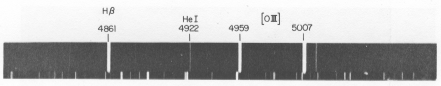
\includegraphics[scale=0.6]{ch3/image7}
	\captionof{figure}{ }
	\end{wrapfigure}

En observant les raies spectrales singulet et triplet, on voit des $O\ II$ : il s'agit des transitions
$M2$ et $E2$ \textit{à priori} interdites mais que l'on voit tout de même (pas le temps d'expliquer
ça malheureusement).

\newpage
\subsection{États doublement excités au-dessus de la limite d'ionisation}

	\begin{wrapfigure}[12]{l}{9cm}
	\vspace{-7mm}
	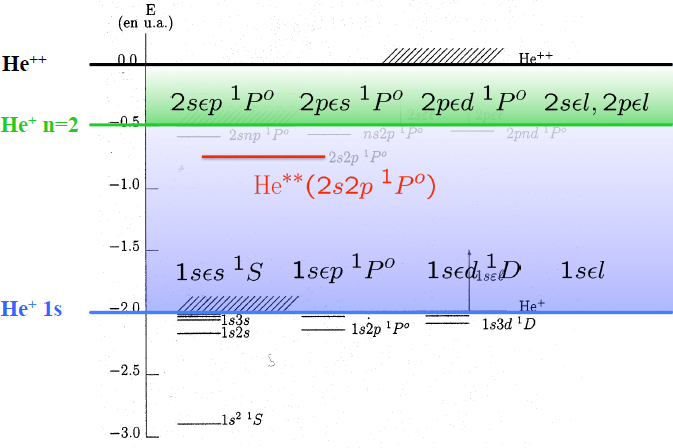
\includegraphics[scale=0.45]{ch3/image8}
	\captionof{figure}{ }
	\end{wrapfigure}
Sur le spectre ci-contre\footnote{Peu de notes sur cette partie.}, on s'intéresse à la partie de
droite (celle de gauche ne comportant pas le fameux terme en $1/r_{12}$). Le cadre, c'est là où
commence l'histoire de l'He$^+$. (lorsqu'un électron est passé "dans le continu").\\

Ce qui est intéressant de constater est que l'état de double excitation est \textbf{en dessous} 
de l'ionisation totale mais au \textbf{dessus} de l'ionisation $He^+$.
 
 
 
\subsection{Résonancesde Madden and Colding (1963)} 
Le \textit{slide 45} illustre la première fois que l'on a réussi à observer l'état doublement 
excité. Il fallaitpour ça exciter l'He fondamental $1s^2$ et aller au delà de la limite d'ionisation.
En bas, on peut voir les raies qui convergent vers l'ionisation (dans les différents états de 
l'He) et un signal continu. \\

Ce qui est à reteniur, c'est l'intéraction entre un état doublement excité (rouge) qui est discret 
($He$ où deux électrons se sont excités) et un continuum (bleu). On dira que l'on a \textit{du rouge
dans un bain de bleu}
\begin{equation}
{\color{red}
 \mbox{He}^{\ast \ast} 
(2snp\; ^1P^o)}
 \leftrightarrow 
{\color{blue}1s \epsilon p \; ^1P^o }
\end{equation}
Pour le comprendre, intéressons-nous à cette double excitation
\begin{equation}
h \nu + \mbox{He}~(1s^2 \; ^1S) \rightarrow \mbox{He}^{\ast \ast} 
(2lnl' \; ^1P^o) 
\rightarrow  \mbox{He}^+ + e^-
\end{equation}
Cette réaction décrit tout d'abord la formation de $He^{**}$ mais ensuite une \textit{autoisonisation}
par émission d'un électron d'\textsc{Auger}.

\begin{center}
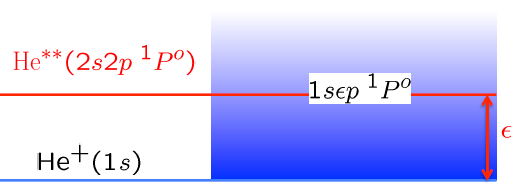
\includegraphics[scale=0.5]{ch3/image9}
\captionof{figure}{Vers la droite \textit{autoionisation} et vers la gauche \textit{capture}}
\end{center}

Nous aurons alors un état $2s2p$ baignant dans un bain bleu continu : cet état va être couplé au 
continu. Cependant, il ne va pas "rester" mais il va s'ioniser afin de libérer un électron. Cette
transition d'un état discret vers un continuum est décrit par la \textit{Fermi Golden Rule} via
\begin{equation}
{\cal{W}}=\frac{2}{\hbar} 
|\langle {\color{blue} \phi_ f} |H'(t)|
{\color{red} \phi_0 } \rangle|^2  {\color{blue} \rho(E_f) }
\end{equation}
qui décrit un profil de \textsc{Fano}. Le \textit{slide 48} décrit les fonctions d'onde du continu
sur lesquelles jene sais pas grand chose à part ce slide.
 
 
\subsection{Structures fines : règle de Landé} 
La structure fine résultat du couplage spin-orbite, rappelons son hamiltonien
\begin{equation}
H^{\mbox{SO}} = \sum_i \xi(r_i) {\bf L}_i \cdot {\bf S}_i\qquad\text{où }\ 
\xi(r_i) = \frac{1}{2 m^2 c^2} \frac{1}{r_i} \frac{dV(r_i)}{dr_i}
\end{equation}
Dans l'atome d'hydrogène, les nombres quantiques $l$ et $s$ n'étaient pas suffisant et il avait 
fallu les coupler pour former $j$. Ici, on va faire de même mais avec $J$ à la place de $j$
\begin{equation}
[H, {\bf J}^2] = [H,J_z] = 0 \Rightarrow 
\left\{
\begin{array}{l}
J = L+S, L+S-1, \ldots, \vert L-S \vert \\
M_J= +J, +J-1, \ldots -J \end{array} \right.
\end{equation}
Dans le cas où nous avons deux électrons, tout ce que nous avons vu pour un seul électron reste vrai,
sauf que dans l'hydrogène \textit{c'était simple\dots}\\

	\begin{wrapfigure}[10]{r}{4.5cm}
	\vspace{-7mm}
	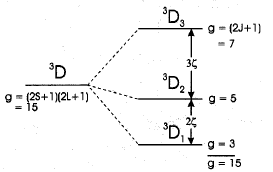
\includegraphics[scale=0.65]{ch3/image10}
	\captionof{figure}{On s'attend expérimentalement à un facteur $3/2$}
	\end{wrapfigure}

Pour faire les choses proprement, il faudrait utiliser la somme définie ci-dessus. Pour avoir une
première idée de ce qui se passe on va utiliser l'approximation suivante
\begin{equation}
{\color{red} \mbox{Si}~H^{\mbox{SO}} 
\approx A \; {\bf L} \cdot {\bf S} }
\end{equation}
Celle-ci fonctionne très bien en physique nucléaire mais malheureusement ses résultats sont moins
bons en physique atomique. L'avantage est que le produit $\vec{L}.\vec{S}$ est facile à traiter
analytiquement. "Sandwichons" cette expression
\begin{equation}
\langle LSJM_J \vert H^{\mbox{S-O}} \vert LSJM_J \rangle =
A \langle LSJM_J \vert {\bf L} \cdot {\bf S} \vert LSJM_J \rangle = \frac{1}{2} A \left[ J(J+1) -
 L(L+1) - S(S+1) \right]
\end{equation}
La différence d'énergie entre un niveau et son niveau inférieur est la règle de \textsc{Landé}\ \\


	
\cadre{\textsc{Règle de Landé} \begin{equation}
E_J - E_{J-1} = A J
\end{equation}}\ \\

Bien évidemment, il existe des écarts expérimentaux à la règle de \textsc{Landé} tout simplement car
\begin{equation}
H^{\mbox{SO}} = \sum_i \xi(r_i) {\bf L}_i \cdot {\bf S}_i
~ {\color{red} \ne  } A \; {\color{red} {\bf L} \cdot {\bf S}  }
\end{equation}
Nous n'avons tout simplement pas considérée la \textit{vraie} interaction mais seulement une 
expression \textit{simplifiée} ce qui exprime une certaine divergence des résultats expérimentaux.


\subsection{Résolution de l'équation de Schrödinger}
Cette partie ne sera pas reprise dans le présent document (elle est principalement technique).


\section{Systèmes complexes et tableau périodique}
Pour des circonstances exceptionnelles, le cours s'arrête fort malheureusement ici.


\iffalse\vspace{4cm}
\begin{center}

\includegraphics[scale=0.2]{ch3/fin}
\end{center}\fi